\subsubsection{12V Speisung}
\label{subsubsec:12V Speisung}

Die Pumpen werden mit 12V betrieben, was zur folge hat, dass eine 12V Speisung implementiert werden musste. Dazu wird ein Schaltspannungsregler verwendet. Dieser wandelt mittels Step-Down Prinzip die 48V des Netzteils in eine konstante Spannung von 12V. Es handelt sich hierbei um einen Regler von Monolithic Power Systems. Genauer gesagt um den MP24943DN-LF. Die Auswahl ist auf dieses Bauteil gefallen, da mit 48V eine relativ hohe Eingangsspannung verarbeitet werden muss. Der MP24943DN-LF kann am Eingang mit Spannungen von 4.5-55V arbeiten und dabei eine Ausgangsspannung von 0.8-45V erzeugen. Dies bei einem maximalen Strom von bis zu 3A. Die Realisierung der 12V Speisung kann in Abbildung \ref{fig:Schema_Speisung_12V} betrachtet werden \cite{\cite{aliexpress_us_nodate}}.\\

\paragraph{Schema}\mbox{}\\

Das Schema in Abbildung \ref{fig:Schema_Speisung_12V} kann in fünf Teile unterteilt werden. Da wären zuerst die Eingangskondensatoren, welche mit C32, C34 \& C36 realisiert sind. Diese Eingangskondensatoren werden gefolgt von einem Spannungsteiler, welcher den Enablepin auf aktiv setzt. Der eigentliche Regler wird mittels des IC7, D6 \& L3 realisiert. Mittels zweier Spannungsteiler, wird die gewünschte Ausgangsspannung, sowie die "Overvoltage-Protection" eingestellt. Vor dem Ausgang der Schaltung ist dann erneut eine Kondensatorstufe implementiert, welche das Ausgangssignal glättet.

\begin{figure}[h!]
	\centering
	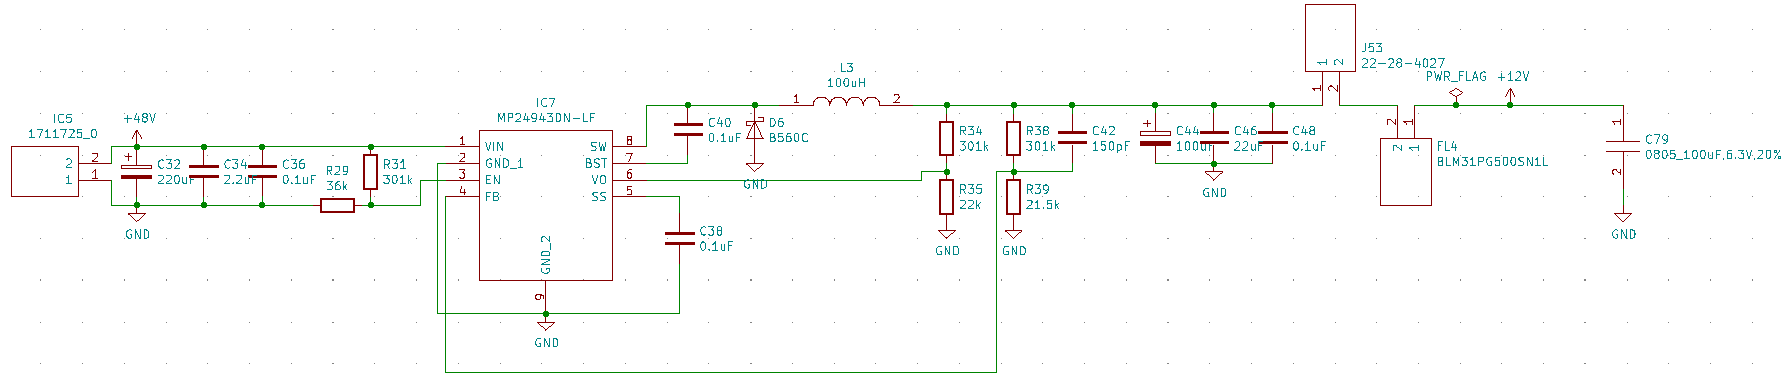
\includegraphics[width=\textwidth]{graphics/Schema_Speisung_12V.png}
	\caption{Schema der 12V Speisung}
	\label{fig:Schema_Speisung_12V}
\end{figure} 

\paragraph{Funktionsbeschrieb der Schaltung}\mbox{}\\

Um den MP24943DN-LF auf aktiv zu setzen, wird eine minimale Spannung von 1.8V vorausgesetzt. Fällt diese unter 0.4V, so wird dieser auf inaktiv gesetzt. Damit der Spannungsregler immer eingeschaltet ist, wird mittels zweier Widerstände R29 \& R31 ein Spannungsteiler realisiert, welcher den Enable (EN) Pin auf 5V und somit auf aktiv setzt. Dieser Spannungsteiler musste implementiert werden, da alle Eingangspins ausser dem V$_{in}$ einen maximale Eingangspegel von 6.5V verkraften können.

Die gewünschte Ausgangsspannung wird mittels Spannungsteiler R39 \& R40 eingestellt, welche auf den Feedback Eingang (FB) rückgekoppelt werden. Diese berechnet sich laut Datenblatt gemäss Formel \ref{equ:Ausgangsspannung_12V}. 

\begin{align}
R40 &= \frac{R39}{\frac{Vout}{0.8}-1}
\label{equ:Ausgangsspannung_12V}
\end{align}

Bei einem Widerstandsverhältnis von R39=301k$\Omega$ \& R40=21.5k$\Omega$ entspricht dies einer Ausgangsspannung von 12V.

Um einer Überspannung vorbeugen zu können, wird am Eingang Voltage-Overshoot (VO) ein Spannungsteiler implementiert. Diese wird am VO-Eingang mit einer Referenzspannung von 0.9V verglichen. Übersteigt die Spannung an VO die Referenzspannung von 0.9V, so wird der Regler ausgeschaltet, bis die Spannung wieder unter 0.9V fällt. Als maximale Ausgangsspannung wurde hierbei eine Spannung von 13V gewählt. Diese Wahl wurde getroffen, da die 12V ausschliesslich für die Ansteuerung der Pumpen verwendet wird und diese eine Spannung von 13V verkraften können ohne Schaden zu nehmen. Der Spannungsteiler wird gemäss Datenblatt mit der Formel \ref{equ:Vovp_12V} berechnet. 

\begin{align}
R35 &= \frac{R34}{\frac{Vovp}{Vovref}-1}
\label{equ:Vovp_12V}
\end{align}

Bei einem Widerstandsverhältnis von R34=301k$\Omega$ \& R35=22k$\Omega$ entspricht dies einer Überspannungsschutzschwelle von 13.21V. 

Der Rippel des Spulenstroms lässt sich gemäss Formel \ref{equ:12V_Spulenberechnung} berechnen. Dieser sollte gemäss Datenblatt ca. 30\% des maximalen Ausgangsstroms von 3A betragen. 

\begin{align}
L3 &= \frac{Vout \cdot (Vin-Vout)}{Vin \cdot \Delta IL \cdot fosc}
\label{equ:12V_Spulenberechnung}
\end{align}

Der interne Oszillator läuft dabei bei einer Frequenz von 100kHz. Bei der ausgewählten Spule von 100$\mu$H erhalten wir ein $\Delta$I$_{L}$ von 0.9A. Ausserdem wird im Datenblatt darauf hingewiesen, dass die gewählte Spule auf mindestens 125\% des maximalen Ausgangsstroms von 3A ausgelegt werden soll. Auch der Gleichstromwiederstand der Spule sollte $ \leq \ $ 200m$\Omega$  sein. 

Mit den Kondensatoren C45, C47 \& C49 wird die Ausgangsspannung zum Abschluss noch geglättet. Bei den Eingangskondensatoren, sowie den Ausgangskondensatoren sollte es sich um low ESR Typen handeln. Um die restlichen hochfrequenten Störungen herauszufiltern, ist zum Abschluss ein Ferrit implementiert worden.

Um die Schaltung einfacher in Betrieb nehmen zu können, wurde mittels Jumper sichergestellt, dass die Speisung vom System abgekoppelt werden kann. Ein LED zeigt an, ob die Speisung funktioniert oder nicht. So ein LED ist jeweils vor und nach dem Jumper implementiert worden. Der Ferrit FL2 soll noch letzte Störungen herausfiltern.

